\documentclass[12pt]{article}
\usepackage[a4paper, margin=1in]{geometry}
\usepackage{graphicx}
\usepackage[backend=biber,style=numeric]{biblatex}
\usepackage[most]{tcolorbox}

\addbibresource{references.bib}

\begin{document}

\author{Joan Ronquillo}

\title{Project Progress - Week 4 of March 2025}
\maketitle

This is a file that contains the tracking of the activities
related to the Hydrodynamic Interactions project during the
fourth week of March 2025. The activities are divided into
groups and a summary of the progress is provided.

\section{Initial Status of the Project}
The project has made significant progress during the third week of March 2025. The key achievements include:
\begin{itemize}
    \item The repository structure has been updated and checked.
    \item The dependencies have been updated in \path{environment.yml}.
    \item The setup.py file has been substituted by a pyproject.toml file, enabling developer mode installation.
    \item Metadata of the modules and packages have been added.
    \item The particles module has been modified with different classes for particle and particle sets.
    \item Fundamental attributes and methods have been added to the classes.
    \item The tests have been updated to check the new classes.
\end{itemize}

So far, the project is developing in some areas:
\begin{itemize}
    \item The development of the Python module with the implementation functions for mobility tensor calculations.
    \item The development of theory to express vectors in VSH basis.
    \item The initial functions to establish specific particle arrangements and geometries.
\end{itemize}

\section{Potential Tasks for the Week}
The following tasks are proposed for this week:
\begin{itemize}
    \item Reading of Raúl's documents on GitHub basics.
    \item Studying the convenience of class/functions for particle arrangements and geometries.
    \item Exploration/creation of Python functions that allow specific particle arrays and geometries to be established.
    \item Exploration/creation of Python functions that handle vector spherical harmonics (VSH) and their properties. Study of the convenience of a class.
    \item Creation of Python functions that allow the mobility tensor to be obtained in the basis of VSH.
    \item Reading of Brenner's paper \cite{BRENNER1961242}.
\end{itemize}

\section{Week Progress}

\subsection{Monday, March 24, 2025}
The SSH connection of the new laptop to the office server
has been successfully configured. The connection name is
"office" and can be accessed using the command "ssh office".
In addition, the connection can be activated from the VSCode
command palette. The particle's module has been updated,
simplifying the particles' class (Structure of Arrays philosophy).
An initial structure for the geometry main class has been created,
yet not tested.

\begin{figure}[h]
    \centering
    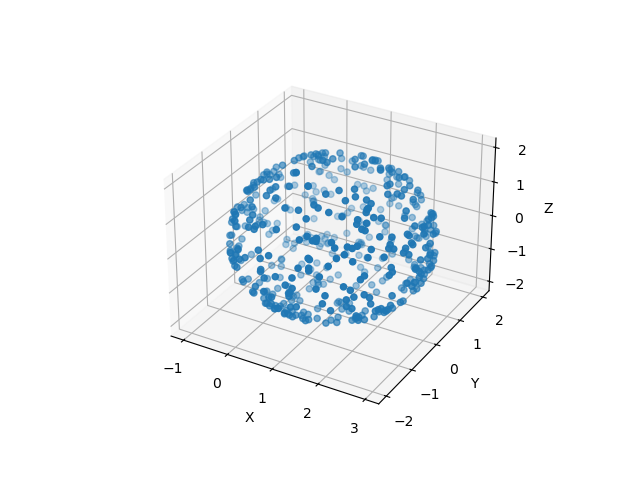
\includegraphics[width=0.8\textwidth]{figures/sphere.png}
    \caption{Plot of a 500 particle sphere.}
    \label{fig:sphere}
\end{figure}

\subsection{Tuesday, March 25, 2025}
The Geometry general class has been tested, and the 
data parameter of the particles' class has been updated.
Now the initialization is better automated and the data
is a list of lists, being each list composed by particle's
properties. A \path{SphereGeometry} subclass has been created
A \path{get_position} method have been added to the geomtry
classes, and plotting and setting position methods have been
added to the particles class. All test have been passed and a
plot of a 500 particle sphere has been created as exposed in
Figure \ref{fig:sphere}.
The graphs and plotting scripts should be moved to a plotting
module, and examples directory or compiled as
commands/executables.

\section{Current Next Steps}
The next steps for the project are:
\begin{itemize}
    \item The managing of plotting outputs
    \item The development of the geometry module.
    \item The development of the VSH module.
    \item Reading of Brenner's paper \cite{BRENNER1961242}.
    \item Reading of Raúl's documents on GitHub basics and documentation generation.
\end{itemize}

\section{Summary}
The project has made significant progress during the fourth
week of March 2025. The key achievements include:


\section {Current Status of the Project}
The project is developing in some areas:


\section{Next Steps}
The next steps for the project are:

\printbibliography

\end{document}
